\documentclass{beamer}
\usepackage{amsmath,amssymb,amsthm,slashed, euscript}
\usepackage{mathrsfs} 

\usepackage{tikz}
\usepackage{tikz-cd}
\usetikzlibrary{cd}

\textwidth=110mm


\title{Algebraic topology of $C^*$-algebras\\ { \fontsize{3}{1} (mathematics and physics)}}
\institute
{
Algebreas in analisys\\
https://arxiv.org/abs/2511.09189
}

\author{Petr R. Ivankov  }



\theoremstyle{plain}
\newtheorem{defn}{Definition}
\newtheorem{rem}{Remark}
\newtheorem{exm}{Example}
\newtheorem*{claim}{Claim}
\newtheorem{prop}{Proposition}
\newtheorem{empt}[prop]{}%[section]
\newtheorem{lem}{Lemma}%[section]
\newtheorem{thm}{Theorem}%[section]

\newcommand{\Dl}{\Delta}
\newcommand{\Z}{\mathbb{Z}}
\newcommand{\A}{\mathcal{A}}
\newcommand{\be}{\begin{equation}}
\newcommand{\ee}{\end{equation}}
	\newcommand{\bean}{\begin{eqnarray*}}
	\newcommand{\eean}{\end{eqnarray*}}
\newcommand{\Ga}{\Gamma}
\newcommand{\B}{\mathcal{B}}
\newcommand{\Cc}{\mathcal{C}}
\newcommand{\C}{\mathbb{C}}
\newcommand{\R}{\mathbb{R}}
\newcommand{\D}{\mathcal{D}}
\newcommand{\G}{\mathcal{G}}
\newcommand{\Hc}{\mathcal{H}}
\newcommand{\Lc}{\mathcal{L}}
\newcommand{\Pc}{\mathcal{P}}
\newcommand{\Sc}{\mathcal{S}}
\newcommand{\U}{\mathcal{U}}
\newcommand{\rar}{\rightarrow}
\newcommand{\Ef}{\mathbb{E}}
\newcommand{\desc}{\mathfrak{desc}}
\newcommand{\rep}{\mathfrak{rep}}
\newcommand{\eps}{\varepsilon}
\newcommand{\T}{\mathbb{T}}


%Uppercase Gothic characters
\newcommand{\gtA}{\mathfrak{A}}
\newcommand{\gtB}{\mathfrak{B}}
\newcommand{\gtM}{\mathfrak{M}}
\newcommand{\gtN}{\mathfrak{N}}
\newcommand{\gtP}{\mathfrak{P}}
\newcommand{\gtS}{\mathfrak{S}}

%Lowercase Gothic characters
\newcommand{\gtf}{\mathfrak{f}}
\newcommand{\gtg}{\mathfrak{g}}

%Bold Characters
\newcommand{\Cb}{\mathbb{C}}
\newcommand{\Nb}{\mathbb{N}}
\newcommand{\Rb}{\mathbb{R}}
\newcommand{\Zb}{\mathbb{Z}}

%Uppercase Greek characters
\newcommand{\Gm}{\Gamma}
\newcommand{\Te}{\Theta}
\newcommand{\Om}{\Omega}
\newcommand{\s}{ }

%Lowercase Greek characters
\newcommand{\al}{\alpha}
\newcommand{\gm}{\gamma}
\newcommand{\dl}{\delta}
\newcommand{\sg}{\sigma}
\newcommand{\ph}{\varphi}
\newcommand{\te}{\theta}
\newcommand{\ze}{\zeta}
\newcommand{\lift}{\mathfrak{lift}}

\newcommand{\Id}{\mathrm{Id}}
\newcommand{\Aut}{\mathrm{Aut}}
\newcommand{\Coo}{{\mathrm{C}}^\infty}
\newcommand{\alg}{\mathrm{alg}}
\newcommand{\diag}{\mathrm{diag}}
\newcommand{\spinc}{\textbf{$spin^c$}}
\newcommand{\Hom}{\mathrm{Hom}}
\newcommand{\supp}{\mathrm{supp}}
\newcommand{\codim}{\mathrm{codim}}
\newcommand{\Ccl}{\mathbf{C}l}
\newcommand{\xto}{\xrightarrow}
	\newcommand{\ga}{\gamma}          %% short for  \gamma

\newcommand{\lto}{\longrightarrow}
\newcommand{\ox}{\otimes}
\newcommand{\nb}{\nabla}
\newcommand{\sS}{\mathcal{S}}
\newcommand{\Dn}{D\!\!\!\!/}
%\newcommand{\ij}{{i,j}}
\newcommand{\aC}{\ensuremath{\underline{\Cb}} }
\newcommand{\scp}[2]{\left\langle{#1},{#2}\right\rangle}
\newcommand{\op}[1]{J{#1}J^\dag}
\newcommand{\K}{\mathcal{K}} 
\newcommand{\F}{\mathcal{F}} 
\newcommand{\E}{\mathcal{E}} 
\newcommand{\sA}{\mathcal{A}} 
\newcommand{\sB}{\mathcal{B}}       %%
\newcommand{\sC}{\mathcal{C}}       %%
\newcommand{\sD}{\mathcal{D}}       %%
\newcommand{\sE}{\mathcal{E}}       %%
\newcommand{\sF}{\mathcal{F}}       %%
\newcommand{\sG}{\mathcal{G}}       %%
\newcommand{\sH}{\mathcal{H}}       %%
\newcommand{\sI}{\mathcal{I}}       %%
\newcommand{\sJ}{\mathcal{J}}       %%
\newcommand{\sK}{\mathcal{K}}       %%
\newcommand{\sL}{\mathcal{L}}       %%
\newcommand{\sM}{\mathcal{M}}       %%
\newcommand{\sN}{\mathcal{N}}       %%
\newcommand{\sO}{\mathcal{O}}       %%
\newcommand{\sP}{\mathcal{P}}       %%
\newcommand{\sQ}{\mathcal{Q}}       %%
\newcommand{\sR}{\mathcal{R}}       %%
\newcommand{\sT}{\mathcal{T}}       %%
\newcommand{\sU}{\mathcal{U}}       %%
\newcommand{\sV}{\mathcal{V}}       %%
\newcommand{\sX}{\mathcal{X}}       %%
\newcommand{\sY}{\mathcal{Y}}       %%
\newcommand{\sZ}{\mathcal{Z}}       %%
\newcommand{\N}{\mathbb{N}}                  %% 
\newcommand{\rank}{\mathrm{rank}}                  %% 

\renewcommand{\a}{\alpha}     
\newcommand{\la}{\lambda}     
\newcommand{\La}{\Lambda}
\newcommand{\bt}{\beta}           %% short for  \beta
\DeclareMathSymbol{\onto}{\mathrel}{AMSa}{"10}
 
    
\newcommand{\bydef}{\stackrel{\mathrm{def}}{=}}  
\newcommand{\hookto}{\hookrightarrow}        %% abbreviation
  
\begin{document}

\begin{frame}
  \titlepage
\end{frame}

\begin{frame}
		{\Large Motivation}
This theory yields $C^*$-algebraic  generalization of algebraic topology invariants which coincide  with invariants of spectrum in case of case of commutative $C^*$-algebras:
\begin{itemize}
	\item (co)homology theory of $\sX$,
	\item $K$-theory  with multiplication and Adams operations.
\end{itemize}
In particular there are followings results:
\begin{itemize}
	\item the Dixmier-Douady obstruction is an obstruction to section of Gelfand space regarded as a bundle over the spectrum,
	\item groups of  $K$-theory  of commutative torus are isomorphic to noncommutative one. However there is no isomorphism of rings. 
\end{itemize}

\end{frame}

\section{Filters and ultrafilters}

%\begin{frame}
	
%	\begin{figure}
%		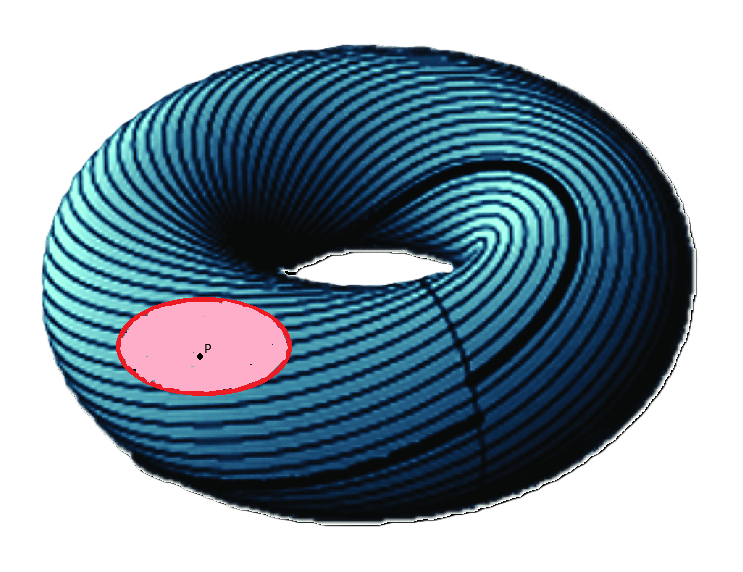
\includegraphics[width=\linewidth]{PICTURE.png}
%		\caption{A boat.}
%		\label{fig:boat1}
%	\end{figure}
%Irrational rotation $C^*$-algebra $C^*_r\left( M, \mathcal F\right)$ and its one-sided ideal.
%end{frame}
\begin{frame}
	
		\begin{definition}\label{upper_defn}
	Let $A$ be a partially ordered set, $S$ a subset of $A$. We say an element $a \in A$
	is a \alert{ meet} (or \alert{ greatest lower bound}) for $S$, and write $a = \wedge S$, if 
	\begin{enumerate}
		\item [(a)] $a$ is an lower bound for $S$, i.e. $a \le s$ for all $s \in S$, and 
		\item [(b)] if $b$ satisfies $\forall \in S\quad  b \le s$, then $b \le a$. 
	\end{enumerate}
	The antisymmetry axiom  ensures that the join of $S$, if it exists, is 
	unique. If $S$ is a two-element set $\{s, t\}$, we write $s \wedge t$ for $\wedge \{s, t\}$ and if $S$	is the empty set $\emptyset$, we write $0$ for  $\wedge \emptyset$.
\end{definition}

\begin{definition}\label{lattice_defn}
	A \alert{meet-semilattice} is a partially ordered set which supports for any finite set the  greatest lower bound.
\end{definition}
\begin{definition}\label{filter_defn}
	A subset $\mathfrak F$ of a meet-semilattice $A$ is said to be an \alert{ filter} if
	\begin{enumerate}
		\item [(a)] $\mathfrak F$ is a sub-meet-semilattice of $A$; i.e. $1\in A$, and $a, b \in \mathfrak F$  imply  	$a \wedge b \in \mathfrak F$; and
		\item [(b)] $\mathfrak F$ is a lower set; i.e. $a \in \mathfrak F$ and $ a\le b$ imply $b \in \mathfrak F$.  
	\end{enumerate}
\end{definition}
\end{frame}
\begin{frame}
		Any homomorphism $\phi : L' \to L''$ of {semi}-{lattices} yields a map
		of filers
		\be\label{filtermap_eqn}
		\left\{I_\la\right\}_{\la \in \La}	\mapsto \text{ minimal filter containing } \left\{\phi\left( I_\la\right) \right\}_{\la \in \La}
		\ee
\begin{definition}\label{ultra_filter_defn}
	A maximal filter is an \alert{ultrafilter}.
\end{definition}		
		\begin{example}\label{space_semi_exm}
			If $\sX$ is a topological space then the $\sX$-\alert{semi}-\alert{lattice} is  a  meet-semilattice $\mathfrak{Lattice}\left( \sX\right)$ such that elements of $\mathfrak{Lattice}\left( \sX\right)$ are open subsets of $\sX$ and one has
			\be\label{x_lat_eqn}
			\begin{split}
				\sU' \wedge \sU''\bydef \sU' \cap \sU'',\\
				\sU' \le \sU'' \quad \Leftrightarrow\quad \sU'' \subset \sU',\\
				0 \bydef \emptyset.
			\end{split}
			\ee
			A set of neighborhoods of a point of Hausdorff space is an ultrafilter.
		\end{example}
	\label{ultra_filter_rem}
			From the Zorn’s lemma it follows that any filter is a subset of an	ultrafilter.

		
	\end{frame}
	\section{Spaces of ultrafilters}
\begin{frame}
\begin{definition}\label{lattice_s_defn}
	If $\mathscr L$ is  the meet-semilattice  then denote by   $\mathfrak{Filters}\left( \mathscr L\right)$  (resp.  $\mathfrak{Ultrafilters}\left( \mathscr L\right)$) the  set of filters  (resp. ultrafilters). \end{definition}
\begin{lemma}\label{topology_l_lem} 
	The set of given by 
	\bean\label{topology_l_eqn}
\mathfrak{Ultrafilters}\left( \mathscr L\right)_L \bydef \left\{ \left.\xi \in \mathfrak{Ultrafilters}\left( \mathscr L\right)\right| L \in \xi\right\}\quad L \in \mathscr L  
	\eean
subsets of $\mathfrak{Ultrafilters}\left( \mathscr L\right)$ 	is a basis of topology.
\end{lemma}
\begin{definition}\label{topology_l_defn} 
	If 	$\mathscr L$ is  a meet-semilattice then the set $\mathfrak{Ultrafilters}\left( \mathscr L\right)$  supplied with the given by the Lemma  topology is the \alert{space of ultrafilters} of $\mathscr L$.
\end{definition}

\end{frame}	
\begin{frame}
		\begin{prop}\label{top_ultra_prop}
	One has:
	\begin{enumerate}
		\item [(a)] 	A topological space $\sX$ is Hausdorff  if and only if every ultrafilter on $\sX$ has at most one limit.
		\item[(b)]   	A topological space $\sX$ is compact if and only if every ultrafilter has at least one limit.
	\end{enumerate} 
\end{prop}
\begin{rem}
From the above proposition it follows that the space of ultrafilters is always compact.
\end{rem}
\end{frame}
\begin{frame}
		{\Large Hausdorff quotients}
	
\begin{definition}\alert{Petr Ivankov}\\
	Let $\sX$ be a topological space. The $\sX$-\alert{Hausdorff category}  $\mathfrak{H}\left( \sX\right)$ is such that 
	\begin{itemize}
		\item objects of $\mathfrak{H}\left( \sX\right)$ are continuous surjective maps $\sX \onto \sY$ onto Hausdorff locally compact  space $\sY$, 
		\item a morphism form $f':\sX \onto \sY'$ to $f'':\sX \onto \sY''$ is a continuous  map  $f: \sY' \onto \sY''$ such that there is the commutative diagram
		\begin{figure}
			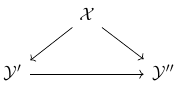
\includegraphics[width=0.5\textwidth]{hauscat.png}
			%		\caption{A boat.}
			%		\label{fig:boat1}
		\end{figure}
		
	\end{itemize}
\end{definition}

\end{frame}
\begin{frame}
\begin{lemma}\alert{Petr Ivankov}\\
	One has:
	\begin{enumerate}
		\item [(i)] for any locally compact topological space $\sX$ there is the natural,   initial object of the  $\sX$-{Hausdorff category} denoted by by $\mathfrak{Hausdorff}\left( \sX\right)$; 
		\item [(ii)] if both $\sX$ and $\sY$ are locally compact spaces then every continuous map $\sX \to \sY$ yields the commutative diagram 	\begin{figure}
			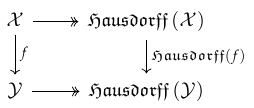
\includegraphics[width=0.5\textwidth]{hausdorff.png}
			%		\caption{A boat.}
			%		\label{fig:boat1}
		\end{figure}
		
		
	\end{enumerate}
\end{lemma}
\end{frame}
\begin{frame}
\begin{definition}\alert{Petr Ivankov}\\
	The initial object of the category $\sX$-{Hausdorff category} is the	$\sX$ - \alert{universal Hausdorff quotient space} denoted by $\mathfrak{Hausdorff}\left(\sX \right)$, 
\end{definition}
\begin{definition}\label{hausdorff_funct_defn}\alert{Petr Ivankov}\\
	The above lemma yields the \alert{Hausdorff functor}
	\be\label{hausdorff_funct_eqn}
	\mathfrak{LocComp} \xrightarrow{\mathfrak{Hausdorff}} \mathfrak{Hausdorff}	\ee
	from the category $\mathfrak{LocComp}$ of locally compact topological spaces and continuous maps to the category of Hausdorff locally compact spaces and continuous maps. 
	\end{definition}
\end{frame}
\section{Gelfand representation}
\begin{frame}
		{\Large Gelfand representation}
	
The \alert{Gelfand representation} is known since 1960s. It yields a generalization of the commutative Gelfand-Na\u{\i}mark theorem.
\begin{definition}\label{open_close_ideal_defn}
	%DEFINITION 11.1. 
Let $A$ be a $C^*$-algebra and $A^{**}$ is its $W^*$-envelope.	A projection $p \in A^{**}$  is \alert{ open} if there exists an increasing 
	net $\left\{a_\la \right\}_{\la \in \La}\subset A_+$ such that $0\ge a_\la \uparrow p$
	$$
	\lim_{\la\in \La} a_\la = p
	$$
	in the weak* topology of $A^{**}$. If $p$ is open, we say $p' \bydef 1=p$ is \alert{closed}.
\end{definition}
\begin{definition}\label{compact_p_defn}
	%DEFINITION ?.l.
	A projection $p\in A^{**}$ is \alert{ compact} if $p$ is {closed}
	and there exists $b \in A_+$ with $bp = p$.
\end{definition}

\end{frame}
\begin{frame}
\begin{definition}\label{coninuous_p_defn}
	%DEFINITION III.2. 
	A self-adjoint operator be $b\in A^{**}$ is \alert{continuous}
	if each spectral projection of $b$ corresponding to an open subset of
	the spectrum of  $b$ is also open.
\end{definition}
The following theorem a generalization of the commutative Gelfand-Na\u{\i}mark theorem.
\begin{theorem}\label{coninuous_p_thm}
	%THEOREM III.3. 
	The self-adjoint elements of $A$ are exactly those
	continuous elements $b$ of $A^{**}$ such that the spectral projections of $b$
	corresponding to closed subsets of the spectrum of $b$ which don't contain
	$0$ are compact (i.e., b "vanishes at $\infty$").
\end{theorem}

\end{frame}

\section{Gelfand space}
\begin{frame}
			{\Large Space of ultrafilters}
	
The commutative  Gelfand-Na\u{\i}mark  theorem yields the equivalence between  following categories:
\begin{itemize}
	\item  unital commutative $C^*$-algebras and $*$-homomorphisms,
	\item compact Hausdorff  spaces and continuous maps.
\end{itemize} 
Here we would like construct a category such that objects of it are all $C^*$-algebras and a functor to the category of locally compact Hausdorff topological  spaces  and continuous maps.
\begin{definition}\alert{Petr Ivankov}\\
	If $A$ is a $C^*$-algebra then $A$-\alert{semi-lattice} $\mathfrak{Lattice}\left( A\right)$ is the meet-semilattice  of open projections of  $A$. We denote by  $\mathfrak{Lattice}\left( A\right)$ the $A$-{semi}-{lattice}.
	A filter (resp, an ultrafilter) of $A$-semi-lattice is an $A$-\alert{filter} (resp. an $A$-\alert{ultrafilter}).	We denote this semilattice by $\mathfrak{Lattice}\left( A\right)$. Denote by $\mathfrak{Filters}\left( A\right)$   the  set of $A$-filters. Denote by $\mathfrak{Ultrafilters}\left( A\right)$ the topological space of ultrafilters of the $\mathfrak{Lattice}\left( A\right)$. 
\end{definition}

\end{frame}
	\begin{frame}
				{\Large Good $*$-homomorphisms}
		For any $C^*$-algebra $A$ there is the natural inclusion $M\left(A \right)  \hookto A^{**}$ of the multiplier into enveloping $W^*$-algebra. For any $C^*$-algebra $B$ a $*$-homomorphism $\varphi :M\left(A \right) \to M\left(B \right)$ induces a homomorphism
		\be\label{w*_eqn} 
		\varphi^{**} : A^{**} \to B^{**}.
		\ee 
		\begin{lemma}\alert{Petr Ivankov}\\
			If both $A$ and $B$ are $C^*$-algebras  and  $\varphi : M\left(  A\right)  \to M\left( B\right) $ is a $*$-homomorphism then for any open projection $p \in A^{**}$  the projection $\varphi^{**}\left( p\right) \in  B^{**}$ is open.
		\end{lemma}
		\begin{rem}
			From the Lemma it turns out that there is the natural continuous map $\mathfrak{Ultrafilters}\left(B\right)\to \mathfrak{Ultrafilters}\left(A \right)$.
		\end{rem}
		
\end{frame}
\begin{frame}
\section{Good $*$-homomorphisms}
\begin{definition}\label{good_hom_defn}\alert{Petr Ivankov}\\
	If both $A$ and $B$ are $C^*$-algebras  then a $*$-homomorphism $\varphi : M\left(  A\right)  \to M\left( B\right) $ is \alert{good} if for any compact projection $q \in B^{**}$ there is a compact projection $p \in A^{**}$ such that
	\be 
	q \le \varphi^{**}\left(p \right). 
	\ee
\end{definition}

\begin{lemma}\alert{Petr Ivankov}\\
	A homomorphism $\varphi: C_b\left( \sX\right) \to C_b\left( \sY\right)$ is good  if and only if  it induces the continuous map  $f: \bt\sY \to \bt\sX$ such that $f\left(\sY \right) \subset \sX$, i.e. there is the natural continuous map $\sY \to \sX$.
\end{lemma}

\end{frame}
\begin{frame}
				{\Large Gelfand spaces}
	
	\begin{definition}\label{gelfand_space_defn}\alert{Petr Ivankov}\\
	If $A$ is a $C^*$-algebra then	an ultrafilter  $\xi = \left\{p_\la\right\}\in \mathfrak{Ultrafilters}\left(A \right)$ is an $A$-\alert{finite point} if there is a nontrivial compact projection $p$  such that $p_\la \wedge  p\neq \{0\}$ for all $\la\in \La$.	The \alert{pre-Gelfand space} $\mathfrak{PreGelfand}\left(A \right)$ of $C^*$-algebra $A$ is a space  of finite points with the final topology  given by the natural inclusion $\mathfrak{PreGelfand}\left(A \right) \hookto \mathfrak{Ultrafilters}\left(A \right)$, where the topology on $\mathfrak{Ultrafilters}\left(A \right)$ is the   Gelfand topology. The \alert{Gelfand space} $\mathfrak{Gelfand}\left(A \right)$ of $C^*$-algebra $A$ is the universal Hausdorff  quotient space of $\mathfrak{PreGelfand}\left(A \right)$ , i.e. $\mathfrak{Gelfand}\left(A \right)\bydef \mathfrak{Hausdorff}\left(\mathfrak{PreGelfand}\left(A \right) \right)$ \end{definition}
	\begin{lemma}\alert{Petr Ivankov}\\
	If $A$ is an unital $C^*$-algebra then both spaces  $\mathfrak{PreGelfand}\left(A \right)\cong \mathfrak{Ultrafilters}\left(A \right)$ and $\mathfrak{Gelfand}\left(A \right)$ are compact. 
\end{lemma}
	
\end{frame}
	\section{Gelfand functor}
\begin{frame}
	\begin{theorem}\alert{Petr Ivankov}\\
	One has
	\begin{enumerate}
		\item [(i)] 	If the  homomorphism $\varphi : M\left( A\right) \to M\left( B\right)$ is good 	  then there are the natural continuous maps
		\bean
		\mathfrak{Gelfand}\left(\varphi \right) :	\mathfrak{Gelfand}\left( B\right) \to \mathfrak{Gelfand}\left( A\right),\\
		\mathfrak{PreGelfand}\left(\varphi \right) :	\mathfrak{PreGelfand}\left( B\right) \to \mathfrak{PreGelfand}\left( A\right) 
		\eean
		
		\item[(ii)] If $\varphi$ is injective then the maps are surjective.
	\end{enumerate}
	
\end{theorem}
\begin{lemma}\alert{Petr Ivankov}\\
	So there is the natural continuous map:
\bean\
\begin{split}
	\mathfrak{Gelfand}\left(A \right) \xrightarrow{\hat \phi} \hat A
\end{split}
\eean
where $\hat A$ is the primitive spectrum.
\end{lemma}

\end{frame}
\begin{frame}
		\begin{definition}\label{gelfand_functor_defn}\alert{Petr Ivankov}\\
		The above theorem  yields  a contravariant \alert{Gelfand functors} 		\bean\label{gelfand_functor_eqn}
		C^*\text{-}\mathfrak{Gelfand}\xrightarrow{\mathfrak{PreGelfand}}\mathfrak{LocComp},\\\label{gelfand_h_functor_eqn}
		C^*\text{-}\mathfrak{Gelfand}\xrightarrow{\mathfrak{Gelfand} \bydef \mathfrak{Hausdorff}~\circ~\mathfrak{PreGelfand}}\mathfrak{Hausdorff}
		\eean
	from	the Gelfand category  to the categories   $\mathfrak{LocComp}$ (resp. $\mathfrak{Hausdorff}$ of locally compact (resp. Hausdorff locally compact) spaces and continuous maps.  
		Any functor  $\mathfrak{LocComp}\to \mathscr C$ and/or $\mathfrak{Hausdorff}\to \mathscr C$ naturally yields the functor $ C^*\text{-}\mathfrak{Gelfand}
		\to \mathscr C$. This circumstance is a motivation of the term "algebraic topology of $C^*$-algebras".
	\end{definition}

\end{frame}
\section{Continuous trace $C^*$-algebras}
\begin{frame}
					{\Large Continuous trace $C^*$-algebras}
	
		\begin{definition}
		A positive element in $C^*$ - algebra $A$ is \alert{Abelian} if subalgebra $xAx \subset A$ is commutative.
	\end{definition}
	\begin{definition}
		%Definition 5.13. 
		A \alert{continuous-trace} $C^*$-\textit{algebra} is a $C^*$-algebra $A$ with Hausdorff
		spectrum $\sX$ such that, for each $x_0\in\sX$ there are a neighbourhood $\sU$ of $x_0$ and $a\in A$ such that $\rep_{ x}\left( a\right) $ is a rank-one projection for all $x \in \sU$.
	\end{definition}
	Let   $A$  be a {continuous-trace} $C^*$-{algebra} with the spectrum $\sX$, and let
	$\mathfrak{Comm}\left( A\right)$ be is a set of all commutative  $C^*$-subalgebras of $A$. For any open $\sU \subset \sX$ let $A_\sU \subset A$ be a $C^*$ -subalgebra such that the spectrum of $A_\sU $ equals to $A_\sU$. Then there is a presheaf  $\mathscr P_{\sX\text{-}A}$  of sets such that for any open $\sU \subset \sX$  one has
	\be\label{presh_eqn}
	\begin{split}
		\mathscr P_{\sX\text{-}A}\left(\sU \right) \left\{ C \in	\mathfrak{Comm}\left( A\right) \left|~ C \subset A_\sU \right. \right\};\\
		\rho_{\sU\sV} : \mathscr P_{\sX\text{-}A}\left(\sU \right)\to \mathscr P_{\sX\text{-}A}\left(\sV \right),\\
		C \mapsto C \cap  A _\sV.
	\end{split}
	\ee
\end{frame}
\begin{frame}
  $\mathrm{Sp\acute{e}}\left(\mathscr P_{\sX\text{-}A} \right)$ be the \'espace etal\'e of the presheaf $\mathrm{Sp\acute{e}}\left(\mathscr P_{\sX\text{-}A} \right)$ with the natural local homeomorphism $p_{\mathrm{Sp\acute{e}}\left(\mathscr P_{\sX\text{-}A} \right)} : \mathrm{Sp\acute{e}}\left(\mathscr P_{\sX\text{-}A} \right) \onto \sX$
\begin{theorem}\alert{Petr Ivankov}\\
	If $A$ is a {continuous-trace} $C^*$-{algebra}  with the spectrum $\sX$ then there is the natural bijective set theoretic map $\phi_{\mathscr P}:\mathfrak{Gelfand}\left( A\right) \cong \mathrm{Sp\acute{e}}\left(\mathscr P_{\sX\text{-}A} \right)$  with the following commutative diagram
\begin{figure}
	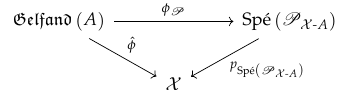
\includegraphics[width=0.5\textwidth]{ctretale.png}
	%		\caption{A boat.}
	%		\label{fig:boat1}
\end{figure}
\end{theorem}	

\end{frame}
\begin{frame}
	\begin{prop}
		%Proposition 9.11 (P. Green [51,96,104]). 
		Let $\sX$ be a second-countable locally compact
		Hausdorff space, and let $A$ and $B$ be stable algebras of continuous trace over $\sX$.
		Then $A \times_\sX B$ is also a stable continuous-trace algebra over $\sX$, and the Dixmier–Douady class $\dl \left(A \otimes_{C_0\left( \sX\right) } B \right)$  of $A \times_\sX B$ is given by $\dl(A) + \dl(B)$. The Dixmier–Douady class of the opposite algebra $A^{\mathrm{op}}$ is given by $\dl\left( A^{\mathrm{op}}\right)=$ - $\dl\left( A\right)$ , so that
		$A\times_\sX  A^{\mathrm{op}}= C_0\left(\sX, \K\right)$.
	\end{prop}
	If both $A$ and $B$ are  stable algebras of continuous trace over $\sX$ with $\dl(A)\neq \dl(B)$ from inclusions  $C_0\left(\sX \right)\subset  M\left( A\right)$  and $C_0\left(\sX \right)\subset  M\left( B\right)$ it turns out that there are surjective continuous maps $\phi_A:\mathfrak{Gelfand}\left( A\right)\onto \sX$ and $\phi_B:\mathfrak{Gelfand}\left( B\right)\onto \sX$. There are homomorphisms then there are homomorphisms $\check{H}^3\left(\mathfrak{Gelfand}\left( \phi_A\right); \Z \right): \check{H}^3\left(\sX; \Z \right) \to \check{H}^3\left(\mathfrak{Gelfand}\left( A\right); \Z \right)$ and $\check{H}^3\left(\mathfrak{Gelfand}\left( \phi_B\right); \Z \right): \check{H}^3\left(\sX; \Z \right) \to \check{H}^3\left(\mathfrak{Gelfand}\left( B\right); \Z \right)$.
\end{frame}
\begin{frame}
	One can prove that $\check{H}^3\left(\mathfrak{Gelfand}\left( \phi_A\right); \Z \right)\left(\dl\left( A\right)  \right) = 0$ and $\check{H}^3\left(\mathfrak{Gelfand}\left( \phi_B\right); \Z \right)\left(\dl\left( B\right)  \right) = 0$. From the above Proposition one has $B = A \otimes_{C_0\left( \sX\right) } C$ with $\dl\left(C \right)  = \dl\left( B\right) - \dl\left(A \right)$. If $a', a \in A$ and $c\in C$ then the equation $a'\left(a \otimes C \right) = a'a\otimes c$ yields the natural action $A\otimes B \to B$. Similarly there is the right action $B \otimes A \to B$. So one has $*$-homomorphisms $A \to M\left( B\right)$, $\varphi: M\left( A\right)\to M\left( B\right)$. There is the following commutative diagram
		\begin{figure}
		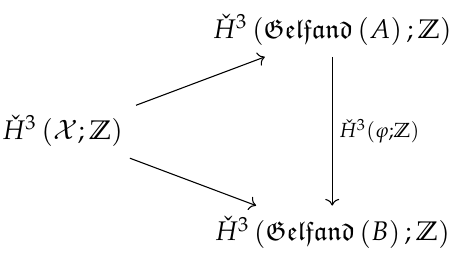
\includegraphics[width=0.5\textwidth]{dd_h3.png}
		%		\caption{A boat.}
		%		\label{fig:boat1}
	\end{figure}
	The homomorphism $\check{H}^3\left(\varphi; \Z \right)$ is not isomorphism since the image of $\dl\left(B \right)$ in  $\check{H}^3\left(\mathfrak{Gelfand}\left( B\right); \Z \right)$ is trivial but the image of  of $\dl\left(B \right)$ in  $\check{H}^3\left(\mathfrak{Gelfand}\left( A\right); \Z \right)$ is not trivial. So the natural surjective map $\mathfrak{Gelfand}\left( B\right)\to \mathfrak{Gelfand}\left( A\right)$ is not isomorphism.
	
	  

\end{frame}
\begin{frame}
		\begin{definition}\alert{Petr Ivankov}\\
		If both  $A$ and $B$ are $C^*$-algebras and $\varphi :M\left(  A\right) \to M\left( B\right)$ is a good $*$-homomorphism then there is a continuous map
		\be\label{gelfand_dd_map_eqn}
		\mathfrak{Gelfand}\left(\varphi \right) :	\mathfrak{Gelfand}\left( B\right) \to \mathfrak{Gelfand}\left( A\right). 
		\ee 
		If $	\mathfrak{Gelfand}\left(\varphi \right) $ is not a homeomorphism then there  is a \alert{generalized Dixmier-Douady obstruction}.
	\end{definition}
\begin{lemma}\alert{Petr Ivankov}\\
	The Dixmier-Douady class is an obstruction to the section $s$  in the following diagram
	following commutative diagram
	\begin{figure}
		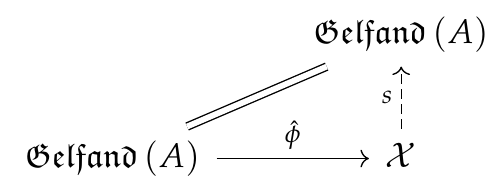
\includegraphics[width=0.5\textwidth]{dd_obstr.png}
		%		\caption{A boat.}
		%		\label{fig:boat1}
	\end{figure}
\end{lemma}	
\end{frame}
\section{Gelfand space and $K$-theory}
\begin{frame}
							{\Large Gelfand space and $K$-theory}
	
Let $A$ be a commutative Banach algebra with maximal ideal space $\sX$.
Then there is a natural homomorphism  $\ga : A \to C_0\left(\sX \right)$, the Gelfand transform induces homomorphisms 
\bean
\ga_*: K_j\left( A\right)\to K_j \left(C_0\left( \sX\right)  \right) \cong K^{-j}\left(\sX \right)\cong K^{j}\left(\sX \right)
\eean
These homomorphisms are actually isomorphisms.
The other isomorphism can then be obtained
using Bott periodicity. The \alert{Shilov Idempotent Theorem} which states that every idempotent in $C_0(\sX)$ is in the image of $\ga$, and hence that the group of integer
linear combinations of idempotents in $A$ is isomorphic to $H^0_c\left(\sX; \Z \right) \cong C_c\left( \sX, \Z\right)$. 
The \alert{Arens-Royden Theorem} states that   an isomorphism
\bean
\text{GL}_1\left(  C_0\left(\sX \right)\right) / \text{GL}_1\left( C_0\left(\sX \right)\right)_0\cong H^1_c\left( \sX, \Z\right)	
\eean

\end{frame}
\begin{frame}
	
		\begin{theorem}
		%	Theorem 2.1. 
		Let $A$ be a Banach algebra (over $\mathbb{F}=\R$ or $\C$). There is a
		functorial "comparison map" of spectra $c : K(A) \to  K^{\mathrm{top}}(A)$ induced by the
		"change of topology" map  $GL\left( A\right)^\dl$ . The induced map $c_* : K_0(A) \to  K_0^{\mathrm{top}}(A)$ is the identity, and the induced map  $c_* : K_0(A) \to  K_0^{\mathrm{top}}(A)$
		is the	quotient map $GL(A/E(A) \to GL(A)/GL(A)_0$. (Here $E(A)$ is the group generated by the elementary matrices, and $GL(A)_0 \supseteq E(A)$ is the identity component of $GL(A)$.)
		Recall also that $K(A)$ is a $K(\mathbb{F})$-module spectrum and that $\mathbb{F}(A)$ is a
		$K_0^{\mathrm{top}}(\mathbb{F})$-module spectrum. The map c is compatible with the product structures,
		in that the diagram
		
	\begin{figure}
		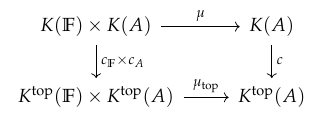
\includegraphics[width=0.5\textwidth]{karoubi_c.png}
		%		\caption{A boat.}
		%		\label{fig:boat1}
	\end{figure}
	
	%	$\mu$ denoting the multiplication maps, is homotopy commutative.
	\end{theorem}	
	
		
\end{frame}
\begin{frame}
	
	\begin{theorem}
		%Theorem 3.3. 
		The Karoubi Conjecture is true for stable $C^*$-algebras, i.e. if $A \cong A \otimes \K$  is a stable $C^*$-algebra, then the comparison map $c : K(A)\to K^{\mathrm{top}}(A)$ of
	above	Theorem  is an equivalence.
	\end{theorem}
\begin{rem}
	If $A$ is a $C^*$-algebra then
	\bean
	K_1\left(A \right) \cong U_1\left(  A \otimes \K \right) / U_1\left( A \otimes \K \right)_0.
	\eean
	If $A$ is a local $C^*$-algebra, then 
	\bean
	\forall n \in \N \quad K_1\left(A \right) \quad \mathrm{GL}_n\left( A \right) / \mathrm{GL}_n\left( A \right)_0\cong U_n\left( A \right) / U_n\left( A \right)_0
	\eean
	
\end{rem}	
\end{frame}

\begin{frame}
		Let $A$ be an unital $C^*$-algebra. If $a \in A$ is a normal element then there is the natural injective $*$-homomorphism $C_0\left( \mathfrak{Sp}_A\left(x \right)\right) \hookto A$. One has the natural surjective continuous map $\varphi : \mathfrak{Gelfand}\left(A  \right) \onto \mathfrak{Sp}_A\left(x \right)$. There is the natural injective $*$-homomorphism $C_0\left( \varphi\right): C_0\left( \mathfrak{Sp}_A\left(x \right)\right) \hookto C\left( \mathfrak{Gelfand}\left(A  \right)\right)$. One can consider $a$ as an element of  $C_0\left( \mathfrak{Sp}_A\left(x \right)\right)$ so one has a map
\bean
\mathfrak{Image}:	a \mapsto b \bydef C_0\left( \varphi\right)\left(a \right) 
\eean
from the set of normal elements of $A$ to $C\left( \mathfrak{Gelfand}\left(A  \right)\right)$. 

\begin{lemma}\alert{Petr Ivankov}\\if $A$ is an unital $C^*$-algebra then one has:
\begin{enumerate}
	\item [(i)]  the  map $\mathfrak{Image}$ is surjective,
	\item[(ii)] there is a one-to-one correspondence between  self-adjoint elements $a \in A$ and bounded real-valued functions $b \in  C\left( \mathfrak{Gelfand}\left(A  \right), \R\right)$.
\end{enumerate}
\end{lemma}
\end{frame}
%\section{Gelfand space and $K$-theory}
\begin{frame}
	
\begin{definition}\label{elementary_defn}
	If $A$ is an unital  $C^*$-algebra then a given by 
	\bean
	\begin{pmatrix}
	a_{1,1}& \ldots & a_{n,1}  \\
	\vdots& \ddots & \vdots\\
	a_{n,1}& \ldots &a_{n,n} \\
\end{pmatrix}	
\eean 
 element $a\in 	 \mathbb{M}_n\left(A \right)$ is  $j,k$-\alert{elementary} if 
	\be\label{elementary_eqn}
	a_{p,q} = \begin{cases}
		1_A & p = j \quad q = k \\
		0 & \text{otherwise}.
	\end{cases}
	\ee
	The  $j,k$-{elementary} element is denoted by
	\be\label{elementary_jk_eqn}
	\mathfrak{e}^{j,k}_A\in \mathbb{M}_n\left(A^+ \right)
	\ee
	
\end{definition}
\end{frame}
\begin{frame}

If $A$ is an unital $C^*$ algebra then the diagonal map 
\bean
	\begin{split}
		d_A : A \hookto \mathbb{M}_n\left(A \right) ,\\
		a \mapsto 		\begin{pmatrix}
			a& \ldots & 0  \\
			\vdots& \ddots & \vdots\\
			0& \ldots &a \\
		\end{pmatrix}
	\end{split}
	\eean
	is a good $*$-homomorphism, it follows that there is a surjective continuous map 
	\bean\label{ge_fc_eqn}
	\begin{split}
		\mathfrak{Gelfand}\left(\mathbb{M}_n\left(A \right)\right) \onto \mathfrak{Gelfand}\left(A \right)
	\end{split}
	\eean
	of compact Hausdorff  spaces, which yields the natural injective $*$-homomorphism
	\bean\label{fin_g_eqn}
	\begin{split}
		C\left( \mathfrak{Gelfand}\left(A \right)\right)  \hookto C\left( \mathfrak{Gelfand}\left(\mathbb{M}_n\left(A \right)\right) \right).
	\end{split}
	\eean
	
\end{frame}

\begin{frame}
\begin{lemma}\alert{Petr Ivankov}\\
If $A$ is an unital $C^*$-algebra $C\left( \mathfrak{Gelfand}\left(\mathbb{M}_n\left(A \right)\right) \right)$ is a finitely generated projective 	$C\left( \mathfrak{Gelfand}\left(A \right)\right)$-module. Indeed there is the natural isomorphism of left $C\left( \mathfrak{Gelfand}\left(A\right)\right)$-modules $C\left( \mathfrak{Gelfand}\left(\mathbb{M}_n\left(A \right)\right)\right) \cong C\left( \mathfrak{Gelfand}\left(A\right)\right) ^n$.
\end{lemma}
If  
$p \in \mathbb{M}_n\left(A \right)$ is a projector then one has the natural disjoint union of open sets
\bean\label{matrppbu_eqn}
\begin{split}
	\mathfrak{Gelfand}\left(\mathbb{M}_n\left(A \right)\right)=\\ \mathfrak{Gelfand}\left(\mathbb{M}_n\left(A \right)\right)_{\mathbb{M}_n\left(A \right)p}\bigsqcup \mathfrak{Gelfand}\left(\mathbb{M}_n\left(A \right)\right)_{\mathbb{M}_n\left(A \right)\left(1_{\mathbb{M}_n\left(A \right)} -p\right) }
\end{split}
\eean
or equivalently
\bean
\begin{split}
	C\left( \mathfrak{Gelfand}\left(\mathbb{M}_n\left(A \right)\right)\right)=\\=	C\left( \mathfrak{Gelfand}\left(\mathbb{M}_n\left(A \right)\right)_{\mathbb{M}_n\left(A \right)p} \right)\bigoplus\\\bigoplus  C\left(  \mathfrak{Gelfand}\left(\mathbb{M}_n\left(A \right)\right)_{\mathbb{M}_n\left(A \right)\left(1_{\mathbb{M}_n\left(A \right)} -p\right) }\right).  
\end{split}
\eean

\end{frame}
\begin{frame}

Both $C\left( \mathfrak{Gelfand}\left(\mathbb{M}_n\left(A \right)\right)_{\mathbb{M}_n\left(A \right)p} \right)$ and $C\left(  \mathfrak{Gelfand}\left(\mathbb{M}_n\left(A \right)\right)_{\mathbb{M}_n\left(A \right)\left(1_{\mathbb{M}_n\left(A \right)} -p\right) }\right)$ are left $C\left(\mathfrak{Gelfand}\left(A \right) \right)$-modules.
i.e. 	$C\left( \mathfrak{Gelfand}\left(\mathbb{M}_n\left(A \right)\right)_{\mathbb{M}_n\left(A \right)p}\right) $ is a finitely generated $C\left(\mathfrak{Gelfand}\left(A \right) \right)$-module. In result one has the following Theorem 
\begin{theorem}\alert{Petr Ivankov}\\
	If $A$ is an unital $C^*$-algebra then one has.
	\begin{enumerate}
		\item [(i)] There is the natural one-to-one correspondence between isomorphism classes of  finitely generated projective $A$-modules and complex vector bundles on the Gelfand space  $\mathfrak{Gelfand}\left(A \right)$.
		\item[(ii)] There is the natural isomorphism
		\bean
		K_0\left( A\right) \cong K^0\left( \mathfrak{Gelfand}\left(A \right)\right). 
		\eean
	\end{enumerate}
	\end{theorem}\end{frame}
\section{$K$-theory of $C^*$-algebra and its Gelfand space}
\begin{frame}
Here we prove that $K$-theory of $C^*$-algebras can be formulated in terms of the sheaf cohomology. If  $A$ is an unital $C^*$-algebra then denote by $\mathfrak{FinProj}\left( A\right)$ the set of finitely generated left $A$-modules. For any $P, Q \in \mathfrak{FinProj}\left( A\right)$ we write $P \sim Q$ if $P$ and $Q$ are isomorphic $A$-modules. The group  $K^{\mathrm{alg}}_0\left( A\right)$ of the algebraic $K$-theory is the universal Abelian group such that
\begin{enumerate}
	\item[(a)]  $\mathfrak{FinProj}\left( A\right)$ is the set of generators of $K^{\mathrm{alg}}_0\left( A\right)$.
	\item[(b)] Foe any pair $P, Q\in \mathfrak{FinProj}\left( A\right)$ satisfy to the following relations:
	\bean
	\left[P \oplus Q\right] = \left[P\right]+\left[Q\right],\\
	P \sim Q \quad \Leftrightarrow \quad \left[P\right]=\left[Q\right]
	\eean
	where $\left[P\right],\left[Q\right], \left[P \oplus Q\right]\in K^{\mathrm{alg}}_0\left( A\right)$ are represented by $P, Q, P\oplus Q$ respectively.
\end{enumerate}
For any   $P \in \mathfrak{FinProj}\left( A\right)$ there is a projection $p \in A \otimes \K$ such that
\bean
P \sim p\left( A \otimes \K\right) 
\eean 

\end{frame}
\begin{frame}
	Following theorem is a consequence of the above construction and Shilov idempotent theorem.
\begin{theorem}\label{k_0_thm}\alert{Petr Ivankov}\\
	If $A$ is an unital $C^*$-algebra then there are following  natural isomorphisms
	\bean\label{k_00_eqn}
	K_0\left( A\right) \cong K_0\left( C\left( \mathfrak{Gelfand}\left(A \right)\right) \right)\cong  H^0_c\left(\mathfrak{Gelfand}\left( A\otimes \K \right); \Z \right)/\sim
	\eean
	where the equivalence relation $\sim$ comes from isomorphism of $C\left( \mathfrak{Gelfand}\left(A \right)\right)$-modules.	
\end{theorem}
\end{frame}
\begin{frame}
Application of the Arens-Royden theorem yields the following.
\begin{theorem}\label{k_1_coh_lem}\alert{Petr Ivankov}\\
	For any unital $C^*$-algebra $A$ there is the natural isomorphism
	\bean
	K_1\left(A \right) \cong U_1\left( A \otimes \K \right) / U_1\left( A \otimes \K \right)_0\cong \\ 	U_1\left( C\left( \mathfrak{Gelfand}\left(  A \otimes \K\right)^+\right)\right)/ U_1\left( C\left( \mathfrak{Gelfand}\left(  A \otimes \K\right)^+\right)\right)_0 \cong \\ \cong H^1_c\left( \mathfrak{Gelfand}\left(  A \otimes \K\right); \Z \right). 
	\eean 
\end{theorem}

\begin{theorem}\alert{Petr Ivankov}\\
	For any   $C^*$-algebra $A$ one has
	\bean
 \quad K_1\left(A \right)  \cong K^1\left(\mathfrak{Gelfand}\left(  A \right) \right).
	\eean
\end{theorem}

\end{frame}

\section{Multiplicative structure}
\begin{frame}
	\begin{lemma}\alert{Petr Ivankov}\\
		For any $C^*$-algebra $A$ and any locally compact Hausdorff space $\sX$ there is the natural homeomorphism
		\bean
		\begin{split}
			\mathfrak{Gelfand}\left(C_0\left(\sX \right)\otimes  A \cong C_0\left(\sX, A \right) \right) \cong \sX \times \mathfrak{Gelfand}\left(A \right),
		\end{split}
		\eean
	\end{lemma}
	From the above Lemma and Bott periodicity one can prove the following theorem
	\begin{theorem}\alert{Petr Ivankov}\\
		For any unital $C^*$-algebra $A$ and every	 $k \ge 0$ one has
			\bean
		K_{r+1~ \mathrm{mod}~2 }\left(A \right) \cong H^1_c\left(S^{r}\mathfrak{Gelfand}\left(A \otimes \K\right); \Z \right)\cong \\ \cong H^1_c\left(\mathfrak{Gelfand}\left(A \otimes \K\right)\times \R^{r}; \Z \right)
		\eean
		for each $r \ge 0$.
	\end{theorem}
	
\end{frame}

\begin{frame}
		{\Large Multiplicative structure} 
			\begin{theorem}
			%15.2. Theorem. 
			(\text{K\"{u}nneth.}) If $\sX$ and $\sY$ are locally compact Hausdorff 
			spaces and if $\mathscr A$ and $\mathscr B$ are sheaves on $\sX$ and $\sY$ respectively with $\mathrm{Tor}_L\left(\mathscr A, \mathscr B \right) = \{0\}$
			then there is a natural exact sequence (over the principal ideal domain $L$
			as base ring)
			\bean
			\begin{split}
				\bigoplus_{p+q = n} H^p_c\left(\sX; \mathscr A \right) \otimes H^q_c\left(\sY; \mathscr A \right)\hookto H^n_c\left(\sX\times \sY; \mathscr A\otimes_L\mathscr B \right)\onto\\ \onto  \bigoplus_{p+q = n+1} \mathrm{Tor}\left( H^p_c\left(\sX; \mathscr A \right),  H^p_c\left(\sX; \mathscr B \right) \right). 
			\end{split}
			\eean
			that splits nonnaturally.	
		\end{theorem}
		
\end{frame}

\begin{frame}
	\begin{theorem}
	%7.1. Theorem. 
	Let $\Phi$ and $\Psi$ be families of supports on $\sX$. Then there exists
	a unique natural transformation of functors (on the category of sheaves on
	X to Abelian groups)
	\bean\label{cup_p_eqn}
	\begin{split}
		\smile : H^p_\Phi\left(\sX, \mathscr A \right) \otimes  H^p_\Psi\left(\sX, \mathscr B \right)\to H^p_{\Phi\cap\Psi}\left(\sX, \mathscr A \otimes \mathscr B\right)
	\end{split}
	\eean
	called the {\it cup product} and satisfying the following three properties:
	\begin{enumerate}
		\item [(a)] For $p = q = 0, ~ \smile \Ga_\Phi\left( \mathscr A\right) \Ga_\Psi\left( \mathscr B\right)\to \Ga_{\Phi\cap \Psi}\left(\mathscr A \otimes \mathscr B \right)$  is the transformation
		induced by the canonical map $\mathscr A\left(\sX\right)\otimes \mathscr B\left(\sX\right)\to \left(\mathscr A \otimes \mathscr A \right)\left(\sX \right)$.   % of I-Section 5.
		\item [(b)] If $0 \hookto \mathscr A' \hookto \mathscr A \onto \mathscr A'' \onto 0$ and $0 \hookto \mathscr A' \otimes \mathscr B\hookto \mathscr A \otimes \mathscr B\onto \mathscr A'' \otimes \mathscr B \onto 0$  , are exact then for $\a \in H^p_\Phi\left(\sX, \mathscr A \right)$ and $\bt \in H^q_\Psi\left(\sX, \mathscr B \right)$ we have $\dl\left( \a \smile \bt\right)= \dl \a  \smile \bt$.
		\item [(c)] If $0 \hookto \mathscr B' \hookto \mathscr B \onto \mathscr B'' \onto 0$ and $0 \hookto \mathscr A \otimes\mathscr B' \hookto\mathscr A \otimes \mathscr B \onto \mathscr A \otimes\mathscr B'' \onto 0$, are exact then for $\a \in H^p_\Phi\left(\sX, \mathscr A \right)$ and $\bt \in H^q_\Psi\left(\sX, \mathscr B \right)$ we have $\dl\left( \a \smile \bt\right)= \left(-1 \right)^p  \a  \smile \dl\bt$.
		
	\end{enumerate}
\end{theorem}
	
\end{frame}
\begin{frame}
	From 
	\be\label{kunnet_sheafrr_eqn}
	\begin{split}
		H^p_c\left(\R^r; \Z \right)= \begin{cases}
			0 & p \neq r,\\
			1 & p = r
		\end{cases}
	\end{split}
	\ee
	it follows that $\sX$ is a locally compact Hausdorff space then one has
	\bean\label{kunnet_sheafr_eqn}
	\begin{split}
		\bigoplus_{p+q = n} H^p_c\left(\sX ; \Z \right) \otimes H^q_c\left(\R^r; \Z \right)\hookto H^{n}_c\left(\sX \times \R^{r}; \Z \otimes \Z \right)\onto\\ \onto  \bigoplus_{p+q = n+1} \mathrm{Tor}\left( H^p_c\left(\sX ; \Z \right),  H^p_c\left(\R^r; \Z \right) \right). 
	\end{split}
	\eean
	
	\bean\label{shift_hom_eqn}
	H^p_c\left( \sX \times \R^k\right) = H^{p + k}_c\left( \sX\right).
	\eean
\end{frame}
\begin{frame}
	There is  the cup  product on the topological $K$-theory given by 
	\bean\label{k_top_p_eqn}
	\begin{split}
		\smile : K^p\left( \sX \right)\times  K^q\left( \sX \right) \to K^{p+q~ \mathrm{mod}~2}\left( \sX \right)
	\end{split}
	\eean
	Here for any unital $C^*$-algebra we find a generalization 
	
	\bean\label{cup_prodcc_eqn}
	\smile : K_p\left(A \right) \otimes K_q\left(A \right) \to K_{p+q~ \mathrm{mod}~2}\left(A \right) \quad \forall p, q \in \{0, 1\}.
	\eean
	of the above product. We will construct the product $\smile : K_p\left(A \right) \otimes K_q\left(A \right) \to K_{p+q~ \mathrm{mod}~2}\left(A \right)$ using the product of sheaf cohomology.
\end{frame}
\begin{frame}
	Suppose that $x \in K_p\left( A\right)$  and $y \in  \in K_q\left( A\right)$ are represented by $u \in H^1_c\left(\mathfrak{Gelfand}\left(A \otimes \K\right)\times \R^{p + 1 + 2n}; \Z \right)$ and $v \in H^1_c\left(\mathfrak{Gelfand}\left(A \otimes \K\right)\times \R^{q + 1 + 2m}; \Z \right)$.
	There is the cup product
	\bean
	u \smile v \in H^2_c\left(\mathfrak{Gelfand}\left(A \otimes \K\right)\times \R^{p+ q + 2 + 2m + 2n}; \Z \right)
	\eean
	The product  $u \smile v$ uniquely defines and element $w \in H^1_c\left(\mathfrak{Gelfand}\left(A \otimes \K\right)\times \R^{p+ q + 1 + 2m + 2n}; \Z \right)$. The element $w$ uniquely defines $z \in K_r\left( A\right)$ such that $p + q = r~\mathrm{mod}~2$;. We define
	\bean
	x \smile y \bydef z.
	\eean 
	It is proven that the product of $K$-theory of topological spaces is a specialization of the above product.
	
	{\bf Conclusion } \alert{The $K$-theory of spaces or/and $C^*$-algebras including their multiplicative structures can be expressed by the cohomology of Gelfand spaces}.\\
		{\bf Question } \alert{Can Adams operations be expressed by the cohomology of Gelfand spaces?}
	
\end{frame}

\section{Gelfand space of noncommutative torus}
\begin{frame}	{\Large Noncommutative torus} 
	\begin{definition}
	Let $\Theta$ be an invertible, real  skew-symmetric quite irrational $n \times n$ matrix. A \alert{noncommutative torus} $C\left(\mathbb{T}^n_{\Theta}\right)$ is the universal $C^*$-algebra generated by the set $\left\{U_k\right\}_{k \in \Z^n}$ of unitary elements which satisfy to the following relations.
	\bean\label{nt_unitary_product_eqn}
		U_k U_j = e^{-\pi ik ~\cdot~ \Theta j} U_{k + j}; ~~~   \
		\eean
\end{definition}
For any $r=1,...,n$ there is the injective  $*$-homomorphism 
\bean
C\left( U_r\right) \hookto C\left(\mathbb{T}^n_{\Theta}\right)
\eean
which yields a continuous surjective map 
\bean
\phi_r\mathfrak{Gelfand}\left(C\left(\mathbb{T}^n_{\Theta}\right)\right)\onto C\left(U_r\right)\cong S^1
\eean 
so there is a continuous map
\bean
\phi : \mathfrak{Gelfand}\left(C\left(\mathbb{T}^n_{\Theta}\right)\right)\to\left(S^1 \right)^n \cong \T^n. 
\eean 
\end{frame}
\begin{frame}
	\begin{lemma}\alert{Petr Ivankov}\\
		The map $\phi : \mathfrak{Gelfand}\left(C\left(\mathbb{T}^n_{\Theta}\right)\right)\to \T^n$ is a bijection.
\end{lemma}
The $C^*$-algebra $C\left(\mathbb{T}^n_{\Theta}\right)$ has \alert{Rieffel projections} $p \in C\left(\mathbb{T}^n_{\Theta}\right)\setminus\{0\}$ i.e. $p^2 = p^*=p$. From the disconnected union 
\bean
\mathfrak{Gelfand}\left(C\left(\mathbb{T}^n_{\Theta}\right)\right) = \mathfrak{Gelfand}\left(C\left(\mathbb{T}^n_{\Theta}\right)\right)_p \bigsqcup \mathfrak{Gelfand}\left(C\left(\mathbb{T}^n_{\Theta}\right)\right)_{1-p}
\eean 
it turns out than the space $\mathfrak{Gelfand}\left(C\left(\mathbb{T}^n_{\Theta}\right)\right)$ is not connected. It is known that there are following isomorphisms of Abelian groups:
\bean
\forall j \in \{0,1\} \quad  K_j\left( C\left(\mathbb{T}^n_{\Theta}\right)\right) \cong K_j\left( C\left(\mathbb{T}^n\right)\right)\cong K^j\left(\T^n \right) \cong \Z^{2^{n-1}}.
\eean 
\end{frame}
\begin{frame}
	\begin{lemma}\alert{Petr Ivankov}\\
			Let  $n = 2k \in \N$ then one has 
		\bean
			K_0\left( C\left(\T^n_{\Theta}\right)\right)  \cong	H^0\left(\mathfrak{Gelfand}\left(C\left(\T^n_{\Theta} \right) \right); \Z \right)\cong   \bigoplus_{j = 1}^{2^{n-1}}\Z s_j,\\
			K_1\left( C\left(\T^n_{\Theta}\right)\right)  \cong	H^1\left(\mathfrak{Gelfand}\left(C\left(\T^n_{\Theta} \right) \right); \Z \right)\cong   \bigoplus_{j = 1}^{2^{n-1}}\Z t_j
		\eean
		where for each $j, k \in \left\{1,..., 2^{n-1}\right\}$ the cup product satisfies to the following equations	
		\bean 
		\begin{split}
			s_j \smile s_k = \begin{cases}
				s_j & j = k\\
				0 & j \neq k
			\end{cases},\\
			s_j \smile t_k = t_k \smile s_j =\begin{cases}
				t_k & j = k\\
				0 & j \neq k
			\end{cases},\\
			t_j \smile t_k = 0.
		\end{split}	
		\eean
		
		
\end{lemma}
 \end{frame}
  \section{Bohr topos}
  
 \begin{frame}
 	{\Large Bohr topos} 
 	The aim of Bohr toposes is to relate algebraic quantum mechanics to
 	topos theory, so as to construct new foundations for quantum logic
 	and quantum spaces.	Bohr toposes provide the topos-theoretical notion of a space which
 	intrinsically carries the intuitionistic logical structure of a Heyting algebra. We need the following.
  	
 	
 	\begin{definition}\label
 		A \alert{frame} is partially  ordered set with all joins and all finite meets which satisfies the infinite distributive law:
 		$$
 		x \wedge \left( \bigvee_\iota y_\iota \right) = \bigvee_\iota\left(x\wedge   y_\iota \right) 
 		$$
 		A \alert{frame homomorphism} 
 		is a function which preserves finite meets and arbitrary joins. Frames and frame homomorphisms form a category $\mathfrak{Frm}$.
 	\end{definition}
 	
 \end{frame}
 \begin{frame}
 	\begin{definition}\label{locale_defn}
 		The category $\mathfrak{ Locale}$ of \alert{locales} is the opposite of the category of frames
 		$$
 		\mathfrak{ Locale} \bydef \mathfrak{Frm}^\text{op}.
 		$$
 		If $X$ is  a locale  denote by $\mathcal O\left( X\right)$ the corresponding  frame.
 	\end{definition}
 	The definition  of sheaves on a topological space depends
 	only on the lattice of open sets of that space, and so extends at once to
 	define sheaves on a locale $X$. Thus an "open" object $U$ is underlying category is said to be
 	covered by a family $\left\{U_\iota \right\}$ of "opens" of $X$ with each $U_\iota \le U$  if and only if $U= \bigvee_\iota V_\iota$ thus
 	\bean\label{localic_site}
 	\left\{U_\iota\subset U \right\} \text{ covers } U \text{ if and only if } U= \bigvee_\iota V_\iota
 	\eean
 	The equation  yields a Grothendieck pretopology, so one obtains a Grothendieck topology. In result we obtain a site and a Grothendieck topos.
 	
\end{frame}
\begin{frame}
\begin{definition}
	Let $X$ be a partially ordered set. We define the \alert{Alexandrov topology} $\Upsilon(X, \le)$ (or simply 
	$\Upsilon(X)$, if the partial order is obvious) to be the collection of all \textit{upper sets}
	in $X$ (i.e. sets $U$ such that $x \in  U$ and $x \le y$ imply $y \in U$); this is clearly a 
	topology, since it is closed under arbitrary unions and intersections. 
	
\end{definition}
\begin{rem}
	The {Alexandrov topology} is not a classical topology, it is Grothendieck topology.
	\end{rem}
\end{frame}
\begin{frame}
	
For any $C^*$-algebra 
one can consider the partially ordered set $\mathcal C(A)$  of commutative
subalgebras of $A$, ordered by inclusion. The assignment of this partially ordered to
a $C^*$-algebra induces a functor $\mathcal C$ from the category of $C^*$-algebras to the category of partially ordered sets, since one has for any
homomorphism $A \xrightarrow{h}B$ a functor $
\mathcal C(A)\xrightarrow{\mathcal C}  \mathcal C(B)$
\begin{figure}
	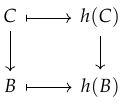
\includegraphics[width=0.3\textwidth]{alex_dgm.png}
	%		\caption{A boat.}
	%		\label{fig:boat1}
\end{figure}
\begin{definition}\label{bohr_topos_defn}
	The \alert{Bohr locale} of $C^*$-algebra $A$ is  an Alexandrov space $L(A)$.
	The \alert{Bohr topos} of $C^*$-algebra $A$ is a  topos sheaves $\mathfrak{Sh}\left( L(A)\right)$ over the Bohr locale.
\end{definition}
\end{frame}
\begin{frame}
\begin{definition}
	
	Let  $A$ be an unital $C^*$-algebra, and let $\mathfrak{Comm}\left( A\right)$ be  the meet-semilattice of commutative $C^*$-subalgebras of $A$. The \alert{ pre-Bohr space} of $A$ (write $\mathfrak{PreBohr}\left(A \right)$ ) is the { space of ultrafilters} of $\mathfrak{Comm}\left( A\right)$.   The \alert{Bohr space} $\mathfrak{Bohr}\left(A \right)$ of $A$ is the universal Hausdorff  quotient space of $\mathfrak{PreBohr}\left(A \right)$, i.e. $\mathfrak{Bohr}\left(A \right)\bydef \mathfrak{Hausdorff}\left(\mathfrak{PreBohr}\left(A \right) \right)$.
\end{definition}
\begin{rem}
The Bohr space is obtained from the Bohr locale by refinement of topology.
\end{rem}
\begin{lemma}\alert{Petr Ivankov}
	If $A$ is an unital $C^*$-algebra then 
one has the natural surjective continuous map
\bean
\mathfrak{Gelfand}\left( A \right)\onto \mathfrak{Bohr}\left( A \right)
\eean
\end{lemma}
 \end{frame}

\begin{frame}
	\alert{Thank you}
\end{frame}


\end{document}























